\chapter{Cronograma}\label{sec:6}

O cronograma é importante pois o mesmo atua como um guia que organiza as atividades, a sua principal metríca é o tempo de entrega de cada uma das atividades. A Figura~\ref{fig:conograma} apresenta o atual cronograma das atividades do projeto.

\begin{figure}[htbp]
    \caption{Conograma}
    \label{fig:conograma}
    \centering
    % O recorte segue a caixa de contorno do conteúdo do PDF, medida com
    % gs -sDEVICE=bbox: 62 59 792 528 numa página de 842x595 pt. Se a imagem
    % for trocada, remeça e ajuste, senão o recorte corta o cronograma.
    \makebox[\textwidth][c]{%
        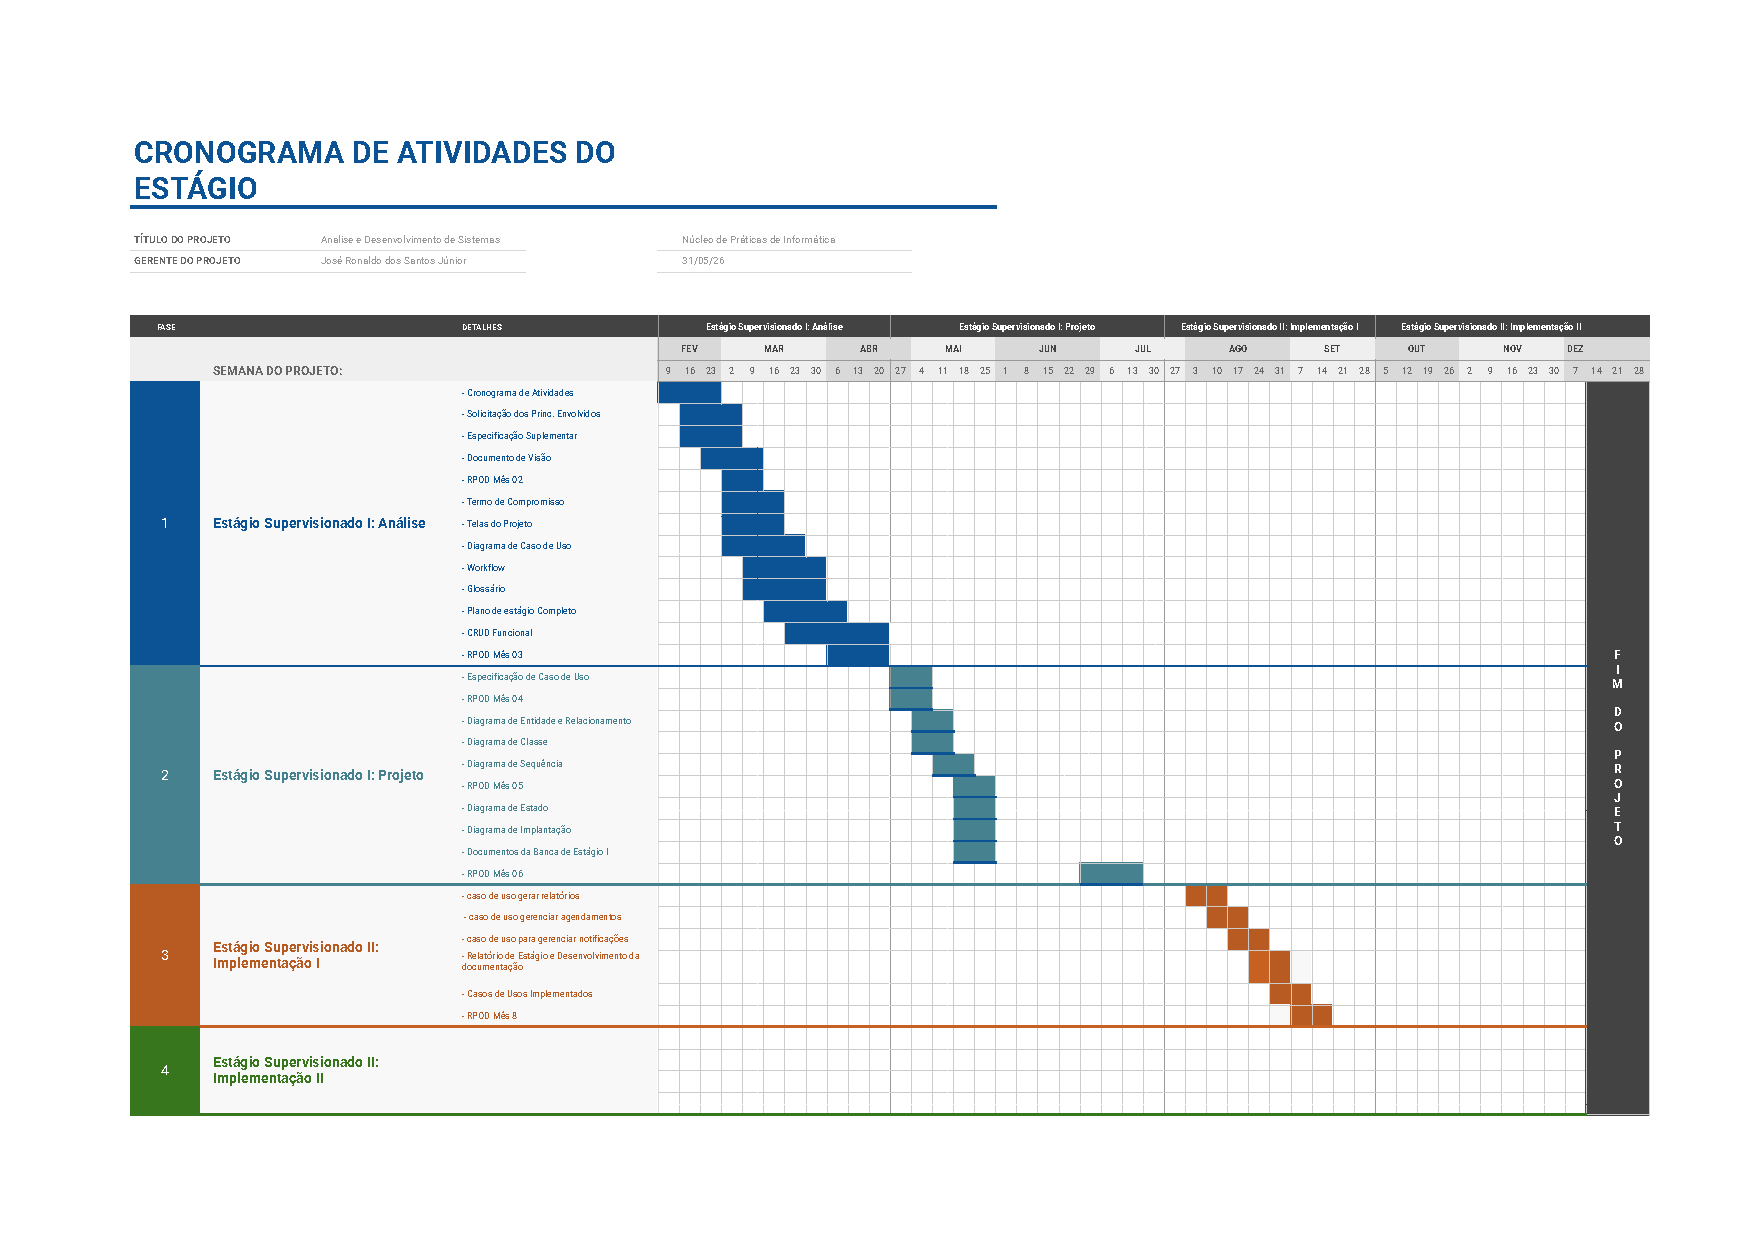
\includegraphics[width=1\textwidth,trim=60 57 48 65,clip]{imagens/CRONO.pdf}
    }
    {\footnotesize \textbf{Fonte:} O autor.}
\end{figure}

% Exemplo de utilização de bibliografia \cite{Gibson2007}.